\documentclass{beamer}
\mode<presentation>
\usepackage{amsmath}
\usepackage{amssymb}
\usepackage{bm}


%\usepackage{advdate}
\usepackage{adjustbox}
\usepackage{subcaption}
%\usepackage{enumitem}
\usepackage{enumerate}
\usepackage{multicol}
\usepackage{mathtools}
\usepackage{listings}
\usepackage{url}
\def\UrlBreaks{\do\/\do-}
\usetheme{Boadilla}
\usecolortheme{lily}
\setbeamertemplate{footline}
{
  \leavevmode%
  \hbox{%
  \begin{beamercolorbox}[wd=\paperwidth,ht=2.25ex,dp=1ex,right]{author in head/foot}%
    \insertframenumber{} / \inserttotalframenumber\hspace*{2ex} 
  \end{beamercolorbox}}%
  \vskip0pt%
}
\setbeamertemplate{navigation symbols}{}

\providecommand{\nCr}[2]{\,^{#1}C_{#2}} % nCr
\providecommand{\nPr}[2]{\,^{#1}P_{#2}} % nPr
\providecommand{\mbf}{\mathbf}
\providecommand{\pr}[1]{\ensuremath{\Pr\left(#1\right)}}
\providecommand{\qfunc}[1]{\ensuremath{Q\left(#1\right)}}
\providecommand{\sbrak}[1]{\ensuremath{{}\left[#1\right]}}
\providecommand{\lsbrak}[1]{\ensuremath{{}\left[#1\right.}}
\providecommand{\rsbrak}[1]{\ensuremath{{}\left.#1\right]}}
\providecommand{\brak}[1]{\ensuremath{\left(#1\right)}}
\providecommand{\lbrak}[1]{\ensuremath{\left(#1\right.}}
\providecommand{\rbrak}[1]{\ensuremath{\left.#1\right)}}
\providecommand{\cbrak}[1]{\ensuremath{\left\{#1\right\}}}
\providecommand{\lcbrak}[1]{\ensuremath{\left\{#1\right.}}
\providecommand{\rcbrak}[1]{\ensuremath{\left.#1\right\}}}
\providecommand{\rank}{\text{rank}}
\theoremstyle{remark}
\newtheorem{rem}{Remark}
\newcommand{\sgn}{\mathop{\mathrm{sgn}}}
\providecommand{\abs}[1]{\left\vert#1\right\vert}
\providecommand{\res}[1]{\Res\displaylimits_{#1}} 
\providecommand{\norm}[1]{\lVert#1\rVert}
\providecommand{\mtx}[1]{\mathbf{#1}}
\providecommand{\mean}[1]{E\left[ #1 \right]}
\providecommand{\fourier}{\overset{\mathcal{F}}{ \rightleftharpoons}}
%\providecommand{\hilbert}{\overset{\mathcal{H}}{ \rightleftharpoons}}
\providecommand{\system}{\overset{\mathcal{H}}{ \longleftrightarrow}}
	%\newcommand{\solution}[2]{\vec{Solution:}{#1}}
%\newcommand{\solution}{\noindent \vec{Solution: }}
\providecommand{\dec}[2]{\ensuremath{\overset{#1}{\underset{#2}{\gtrless}}}}
\newcommand{\myvec}[1]{\ensuremath{\begin{pmatrix}#1\end{pmatrix}}}
\newenvironment{amatrix}[1]{%
  \left(\begin{array}{@{}*{#1}{c}|c@{}}
}{%
  \end{array}\right)
}
\let\vec\mathbf

\lstset{
%language=C,
frame=single, 
breaklines=true,
columns=fullflexible
}

%\numberwithin{equation}{section}

\title{Matgeo-4.2.2}
\author{Harichandana Varanasi-ai25btech11039}

\date{\today} 
\begin{document}

\begin{frame}
\titlepage
\end{frame}

\section*{Outline}

\begin{frame}
\frametitle{Question}

\textbf{Q-4.2.2} 

Find the direction and normal vectors of the line
\begin{align*}                 
    x - \frac{y}{5} - 10 = 10
\end{align*}




\end{frame}
%
\begin{frame}

\setcounter{equation}{0}
\renewcommand{\theequation}{\arabic{equation}}
Find the direction and normal vectors of the line
\begin{align}
    x - \frac{y}{5} - 10 &= 10
    \label{eq1}
\end{align}

Rewriting \eqref{eq1},
\begin{align}
    x - \frac{y}{5} &= 20
    \label{eq2}
\end{align}

Comparing with the standard form
\begin{align}
    \vec{n}^T\vec{x} &= c,
    \label{eq3}
\end{align}
we obtain
\begin{align}
    \vec{n} = \myvec{1 \\ -\tfrac{1}{5}}, \quad
    \vec{x} = \myvec{x \\ y}, \quad
    c = 20
    \label{eq4}
\end{align}



\end{frame}
\begin{frame}{Solution}


   Thus, the normal vector is
\begin{align}
    \vec{n} = \myvec{1 \\ -\tfrac{1}{5}}
    \label{eq5}
\end{align}

From the orthogonality condition,
\begin{align}
    \vec{m}^T\vec{n} = 0
    \label{eq6}
\end{align}

Let
\begin{align}
    \vec{m} = \myvec{1 \\ 5}
    \label{eq7}
\end{align}
which satisfies \eqref{eq6}.




\end{frame}
\begin{frame}{Solution}

  Hence, the required vectors are
\begin{align}
    \text{Direction vector: } \vec{m} = \myvec{1 \\ 5} \label{eq8}\\
    \text{Normal vector: } \vec{n} = \myvec{1 \\ -\tfrac{1}{5}} \label{eq9}
\end{align}  

    
\end{frame}
\begin{frame}{Plot}
    
\begin{figure}[h!]
\centering
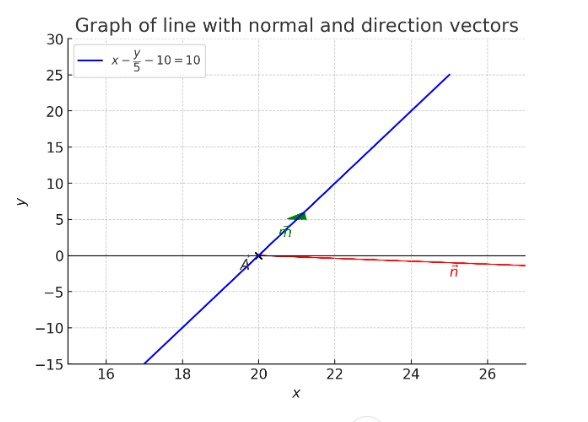
\includegraphics[width=0.5\linewidth]{figs/matgeo 4.2.2.jpeg}
 \caption{Line $x - \tfrac{y}{5} - 10 = 10$ with direction $\vec{m}$ and normal $\vec{n}$.}
    \label{fig:4.2.2}
\end{figure}
\end{frame}

\end{document}
